%!TEX encoding = UTF-8 Unicode
\documentclass[preprint,12pt]{elsarticle}

\usepackage{booktabs}
\usepackage{multirow}
\usepackage{makecell}
\usepackage{graphicx}
\usepackage{adjustbox}
\usepackage{subcaption}
\usepackage{amsmath,amssymb,amsfonts,amsthm}
\usepackage{listings}
\usepackage{xcolor}
\usepackage{microtype}
\usepackage{enumitem}
\usepackage{tikz}
\usepackage{pgfplots}
\usepackage{hyperref}

\pgfplotsset{compat=1.18}
\usetikzlibrary{shapes.geometric,arrows.meta,positioning,fit,backgrounds,calc}
\setlist{nosep,leftmargin=*}

\newtheorem{proposition}{Proposition}

% Absorb small residual overfull boxes from long hyphenated compound terms.
\emergencystretch=3em

% Set the elsarticle preprint footer one size smaller so the
% "Preprint submitted to ...\hfill<date>" line fits within \textwidth.
\makeatletter
\def\ps@pprintTitle{%
  \let\@oddhead\@empty
  \let\@evenhead\@empty
  \def\@oddfoot{\scriptsize\itshape Preprint submitted to \@journal\hfill\today}%
  \let\@evenfoot\@oddfoot}
\makeatother

\newcommand{\oasisUseMaxWidthResize}[1]{%
  \renewcommand{\resizebox}[3]{\adjustbox{max width=#1}{##3}}%
}

% Subheadings upright bold instead of elsarticle's default italic (cosmetic only; the
% final Elsevier typesetting is unaffected). Spacing values copied verbatim from
% elsarticle.cls; only the font shape \itshape is swapped for \bfseries, and the
% \paragraph run-in period mechanism is left intact.
\makeatletter
\renewcommand\subsection{\@startsection{subsection}{2}{\z@}%
           {12\p@ \@plus 6\p@ \@minus 3\p@}%
           {3\p@ \@plus 6\p@ \@minus 3\p@}%
           {\normalfont\normalsize\bfseries}}
\renewcommand\subsubsection{\@startsection{subsubsection}{3}{\z@}%
           {12\p@ \@plus 6\p@ \@minus 3\p@}%
           {\p@}%
           {\normalfont\normalsize\bfseries}}
\renewcommand\elsparagraph{\@startsection{paragraph}{4}{0\z@}%
           {10\p@ \@plus 6\p@ \@minus 3\p@}%
           {-6\p@}%
           {\normalfont\bfseries}}
\makeatother

\lstset{
  basicstyle=\ttfamily\scriptsize,
  breaklines=true,
  frame=single,
  numbers=left,
  numberstyle=\tiny,
  keywordstyle=\color{blue!70!black}\bfseries,
  commentstyle=\color{gray},
  stringstyle=\color{teal},
}

\journal{a database systems journal}% TODO: set target venue (e.g. TODS / VLDB Journal / TKDE) before submission

\begin{document}

\begin{frontmatter}

\title{OASIS: Repairing Stale and Correlation-Blind Query-Optimizer Statistics from Query Feedback}

\author[inst1]{Qichu Tian\corref{cor1}}
\ead{mizukiqwq@stu.xjtu.edu.cn}

\author[inst1]{Heng Chen}
\ead{hengchen@xjtu.edu.cn}
\cortext[cor1]{Corresponding author}

\address[inst1]{Xi'an Jiaotong University, Xi'an, China}

\begin{abstract}
Cost-based optimizers plan with column statistics that drift stale between refreshes and
that assume columns are independent; both errors mislead the planner. Query execution
already exposes them---for every filter predicate the executor reveals the selectivity the
optimizer mis-estimated---so we ask how far query feedback alone, without rescanning the
table, can maintain optimizer-facing statistics. We separate two regimes.

For a \emph{single} column, feedback determines the marginal up to a small free part, and a
maximum-entropy projection (the classical ISOMER step) is already near-optimal: we give an
identifiability condition for when feedback pins the marginal, and show on real datasets,
against self-tuning histograms and a learned prior, that nothing beats the projection
there---single-column repair is easy. The optimizer's larger residual error is the
\emph{independence assumption} on correlated columns, and there feedback helps decisively: a
feedback-driven joint repair cuts conjunctive-predicate Q-error by up to $31\%$ ($13.6\%$ in
aggregate) over independence on real correlated columns, the gain concentrated where
the columns are correlated.

We package this as OASIS, a statistics-layer
middleware that maintains optimizer statistics from query feedback between full
\texttt{ANALYZE} refreshes. Injected into a real PostgreSQL planner, feedback-maintained
single-column statistics cut row Q-error from $27.8$ to $2.4$ and lift fresh-plan match from
$56\%$ to $96\%$ without a table scan, and the maintained marginals stay safe for
composition and join estimators to consume.
\end{abstract}

\begin{keyword}
Cardinality estimation \sep Query optimization \sep Self-tuning histograms
\sep Independence assumption \sep Query feedback \sep Statistics maintenance
\end{keyword}

\end{frontmatter}

\section{Introduction}
\label{sec:intro}

Cost-based optimizers (CBOs) choose query plans from estimates of predicate
selectivity, intermediate cardinality, and operator cost
\cite{selinger1979access,chaudhuri1998overview}. In many analytical database
systems these estimates rely on column-level statistics such as histograms,
most-common-value lists, and density summaries
\cite{ioannidis1993histogram,poosala1997selectivity,postgresqlPlannerStats,postgresqlRowEstimation},
refreshed periodically by \texttt{ANALYZE}-style procedures that read a full or
sampled view of the table~\cite{postgresqlAnalyze}. This maintenance strategy is
simple and robust, but it leaves a persistent staleness gap: tables keep receiving
inserts, deletes, and updates while the optimizer plans with the last statistics
snapshot. As the gap widens, stale histograms induce systematic selectivity errors
that propagate through the cost model into poor plans
\cite{leis2015good,moerkotte2009preventing,han2021cardinality,lee2023impact}. A second,
orthogonal error is structural rather than temporal: per-column statistics carry no
cross-column information, so the optimizer falls back on the attribute-value-independence
assumption and systematically mis-estimates conjunctions over correlated columns
\cite{poosala1997selectivity,leis2015good}.

A DBMS already obtains the signal to repair both errors while executing ordinary queries.
For a filter predicate, the optimizer's estimated and the executor's observed selectivity
expose a local discrepancy between the stale statistics and the current data; for a
conjunction over several columns, the same feedback reveals the joint selectivity the
independence assumption got wrong. Feedback-driven self-tuning histograms turn such
observations into statistics updates---STHoles, SASH, and ISOMER are the canonical examples
\cite{aboulnaga1999self,bruno2001stholes,lim2003sash,markl2007consistent}---and ISOMER makes
the principle explicit: among all distributions consistent with the observed feedback, choose
the \emph{maximum-entropy} one---the least-committed completion of the part feedback leaves
undetermined.

This paper asks a deployment question: \emph{how far can query feedback alone, with no table
rescan, maintain the statistics a cost-based optimizer actually plans with?} The answer
splits cleanly into two regimes, and that split is the organizing idea.

\emph{Single columns are easy.} An equi-depth histogram with $B$ buckets has only $B-1$ free
interior boundaries; a feedback window pins the cumulative distribution at the observed
boundaries and leaves a small free part. We make this precise with an identifiability
condition (Section~\ref{sec:mechanism}) for when feedback determines the marginal, and we
find empirically---on real datasets, against self-tuning histograms and against a prior
trained directly on the optimizer's error---that once the feedback projection is applied,
\emph{nothing beats the maximum-entropy completion}: a learned model gives no edge over the
classical ISOMER step. Single-column repair therefore needs no machine learning; the
principled projection suffices, and we prove and measure when it does.

\emph{Independence is the bottleneck.} The optimizer's larger residual error is the
independence assumption introduced above. Maximum entropy over a single column cannot touch
it, but conjunctive feedback can---it directly observes the joint mass independence gets
wrong. A feedback-driven joint repair (a two-dimensional max-entropy projection onto
observed conjunctive masses) cuts conjunctive-predicate Q-error by up to $31\%$---$13.6\%$ in
aggregate---over the independence assumption on real correlated columns, with the gain
concentrated where the columns are correlated (Section~\ref{sec:crosscol}). This is where feedback
maintenance earns its keep for the optimizer.

The resulting system is OASIS, a
statistics-layer middleware that maintains optimizer statistics from query feedback between
full \texttt{ANALYZE} refreshes, with no base-table rescan. A \emph{conversion layer} maps
native engine statistics to a canonical distribution view and back
(Section~\ref{sec:mcv-adapter}); a \emph{repair layer} applies the feedback-consistency
projection---to a single marginal, and, for correlated columns, to the joint
(Sections~\ref{sec:stage2}, \ref{sec:crosscol}); and a \emph{safety layer} routes among
candidate corrections on a deployment-visible signal so an imperfect correction never
degrades below the maximum-entropy default (Section~\ref{sec:stage2}). Because the correction
is inserted at the statistics layer, the optimizer's search and cost model are untouched.
This design yields four contributions:
\begin{itemize}
  \item An \emph{identifiability} analysis of feedback-driven repair: a rank condition
        (Proposition~\ref{prop:pinned}) for when query feedback pins the optimizer-relevant
        statistic, and when it leaves a free part no consistent method can resolve from
        feedback alone (Sections~\ref{sec:problem}, \ref{sec:mechanism}).
  \item A clean \emph{dichotomy}, validated on real data: single-column repair is
        easy---the maximum-entropy projection is near-optimal, and a learned prior and the
        self-tuning histograms STHoles and QuickSel-H give no edge over it
        (Section~\ref{sec:single-column-results})---whereas the independence assumption is
        the dominant residual optimizer error.
  \item A \emph{feedback-driven independence repair} that beats the
        attribute-value-independence assumption by up to $31\%$ ($13.6\%$ aggregate) on real
        correlated columns, with the gain concentrated where the columns are correlated
        (Section~\ref{sec:crosscol}).
  \item \emph{OASIS}, a no-rescan statistics-maintenance middleware validated in a real
        PostgreSQL planner---feedback-maintained single-column statistics cut row Q-error
        from $27.8$ to $2.4$ and lift fresh-plan match from $56\%$ to $96\%$---with the
        maintained marginals shown safe for composition and join estimators to consume and a
        residual-gated router that never degrades below the maximum-entropy default
        (Section~\ref{sec:optimizer-facing}).
\end{itemize}

\section{Background and Problem Formulation}
\label{sec:background}

\subsection{Feedback-Based Statistics Maintenance}
\label{sec:scenario}

Because an \texttt{ANALYZE}-style refresh must read a full or sampled view of the table,
refreshes are scheduled rather than continuous; between them the table keeps changing
while the optimizer plans from the last snapshot, so a once-accurate histogram drifts from
the current distribution---especially around recent values, range predicates, and
localized updates.

Query execution already exposes this drift: for each filter predicate, the optimizer's
estimated selectivity and the executor's observed selectivity reveal a local disagreement
between the old statistics and the current data.
Feedback-driven self-tuning histograms use such observations to repair statistics: STHoles
splits and refines buckets from feedback~\cite{bruno2001stholes}; ISOMER selects the
maximum-entropy histogram among those consistent with the feedback and drops old
constraints when drift makes the active set inconsistent~\cite{markl2007consistent};
QuickSel-H fits a query-driven selectivity model on the same no-rescan interface
\cite{park2020quicksel}. These methods all take query feedback as input and emit a
corrected single-column statistic without touching the base data. Their key difference is
how they complete the parts of the distribution that feedback does not determine. OASIS
keeps the same interface and the same maximum-entropy completion for a single column; its
leverage is extending the feedback projection to the cross-column joint and routing among
candidates for safety.

\subsection{Statistics and Objective}

We model a column histogram as an equi-depth quantile summary with $B$ buckets. Its
interior boundaries $v_1,\ldots,v_{B-1}$ correspond to fixed quantile levels
$p_1,\ldots,p_{B-1}$ and induce a piecewise-linear CDF used to estimate range-predicate
selectivity. Native DBMS statistics may also include most-common-value lists, density
vectors, or null fractions; OASIS operates on a canonical one-dimensional CDF view and
converts to and from native statistics through an engine-specific adapter
(Section~\ref{sec:mcv-adapter}).

Let $H_0$ be the stale histogram from the last refresh and $H^\ast$ the current
post-drift distribution. For a predicate $\sigma$, the optimizer derives an estimate
$\hat{s}_{H_0}(\sigma)$ from $H_0$, while the executor can later reveal an actual
selectivity $s^\ast(\sigma)$. A feedback window
$\mathcal{O}=\{o_1,\ldots,o_K\}$ records such observations; each $o_j$ contains a
predicate type, a boundary, an estimated selectivity, and an actual selectivity. We
measure error with Q-error,
\begin{equation}
  \mathrm{QErr}(\hat{s},s^\ast) =
  \max\!\left(\frac{\hat{s}}{s^\ast}, \frac{s^\ast}{\hat{s}}\right).
  \label{eq:qerr}
\end{equation}
For one predicate, Q-error is a scalar. To compare two statistics objects, we average
this scalar over future predicates. Let $\sigma\sim\mathcal{D}_{\mathrm{fut}}$ denote a
future predicate drawn from the workload distribution, and let $s^\ast_{\sigma}$ be its
true selectivity under the current distribution $H^\ast$. The goal is to construct
corrected statistics $\hat{H}$ that lower this average future-predicate error,
\[
  \mathbb{E}_{\sigma\sim\mathcal{D}_{\mathrm{fut}}}\!\left[
    \mathrm{QErr}\!\left(\mathrm{CDF}_{\hat{H}}(\sigma),s^\ast_{\sigma}\right)
  \right]
  <
  \mathbb{E}_{\sigma\sim\mathcal{D}_{\mathrm{fut}}}\!\left[
    \mathrm{QErr}\!\left(\mathrm{CDF}_{H_0}(\sigma),s^\ast_{\sigma}\right)
  \right].
\]
A deployable repair must derive $\hat{H}$ from $H_0$ and feedback only, avoid table
rescans, run near planning time, and degrade gracefully when feedback is sparse.

\subsection{Degrees of Freedom in Feedback-Based Repair}
\label{sec:problem}

Feedback repair is underdetermined for an elementary reason. A feedback window reports the
true mass on a handful of intervals; between and beyond those intervals, the data can be
arranged in many ways and still reproduce every observation. The repaired marginal is thus
\emph{pinned} where feedback falls and \emph{free} everywhere else, and that free
part (Figure~\ref{fig:nullspace}) is what any repair method must fill. We make this precise
and measure how large the free part is below.

\begin{figure}[t]
  \centering
  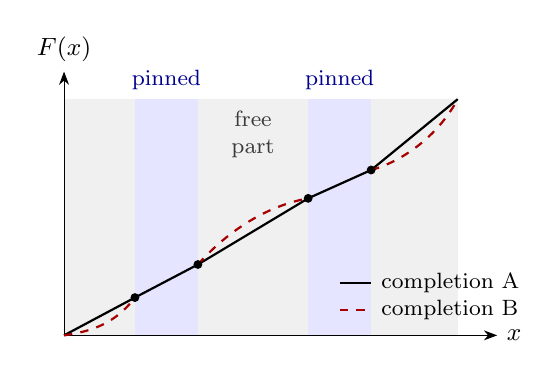
\begin{tikzpicture}[font=\small,>=Stealth]
    % regions the feedback leaves free (the free part)
    \fill[gray!12] (0,0) rectangle (0.9,3.0);
    \fill[gray!12] (1.7,0) rectangle (3.1,3.0);
    \fill[gray!12] (3.9,0) rectangle (5.0,3.0);
    % intervals the feedback pins
    \fill[blue!10] (0.9,0) rectangle (1.7,3.0);
    \fill[blue!10] (3.1,0) rectangle (3.9,3.0);
    % axes
    \draw[->] (0,0) -- (5.5,0) node[right]{$x$};
    \draw[->] (0,0) -- (0,3.35) node[above]{$F(x)$};
    % one consistent completion (solid, piecewise-linear CDF through the anchors)
    \draw[thick] (0,0) -- (0.9,0.48) -- (1.7,0.90) -- (3.1,1.74) -- (3.9,2.10) -- (5.0,3.0);
    % another consistent completion (dashed): differs only in the free regions
    \draw[thick,dashed,red!65!black] (0,0) .. controls (0.35,0.05) and (0.65,0.15) .. (0.9,0.48);
    \draw[thick,dashed,red!65!black] (1.7,0.90) .. controls (2.1,1.35) and (2.6,1.65) .. (3.1,1.74);
    \draw[thick,dashed,red!65!black] (3.9,2.10) .. controls (4.2,2.18) and (4.7,2.45) .. (5.0,3.0);
    % cumulative values pinned by feedback
    \foreach \p in {(0.9,0.48),(1.7,0.90),(3.1,1.74),(3.9,2.10)} \fill \p circle (1.6pt);
    % labels
    \node[blue!55!black,font=\footnotesize,above] at (1.3,3.0) {pinned};
    \node[blue!55!black,font=\footnotesize,above] at (3.5,3.0) {pinned};
    \node[gray!45!black,font=\footnotesize,align=center] at (2.4,2.55) {free\\part};
    % legend
    \draw[thick] (3.5,0.66) -- (3.9,0.66) node[right,font=\footnotesize]{completion A};
    \draw[thick,dashed,red!65!black] (3.5,0.32) -- (3.9,0.32) node[right,font=\footnotesize,text=black]{completion B};
  \end{tikzpicture}
  \caption{Why feedback repair is underdetermined. A feedback window pins the cumulative
  mass $F$ at the predicate boundaries it observes (dots); on the pinned intervals (blue)
  every consistent completion agrees, but on the regions the feedback leaves free
  (grey)---the free part---completions may differ (solid versus dashed) while still matching
  every observation---so the free regions are exactly what any repair method must fill, and once
  feedback pins them no choice remains (Section~\ref{sec:mechanism}).}
  \label{fig:nullspace}
\end{figure}

To make this precise, we rewrite the feedback constraints in a
representation that makes them \emph{exactly linear}. Take the active feedback predicates
together with the stale histogram grid; their boundary points---the grid points and the
distinct feedback endpoints---partition the domain into $C$ cells. We then represent the
marginal by its vector of cell masses $m\in\Delta$. Since these $C$ masses are nonnegative
and sum to one, the simplex $\Delta$ has dimension $C-1$.

In this \emph{cell-mass representation}, each feedback observation constrains only the
total mass on its predicate interval. Because every predicate endpoint is a cell boundary,
that interval mass is an exact sum of cell masses (two such sums for a
\texttt{BETWEEN}). The feedback window therefore imposes a system of linear equality
constraints $A m = y$, with $A\in\mathbb{R}^{K'\times C}$. Let
$r=\mathrm{rank}(A)$. The marginals consistent with the feedback form the affine slice
$\{m\in\Delta : A m = y\}$, whose free dimension is $(C-1)-r$. We call this the
\emph{free subspace} that the feedback leaves.

A deployed histogram exposes only $B-1$ of these $C$ cell boundaries, and on a fixed grid
the two representations are interchangeable---inverting the implied CDF recovers the cell
masses from the exposed quantiles. Section~\ref{sec:mechanism} therefore measures an
\emph{operational} rank on those $B-1$ boundaries---a deployable proxy for
$\mathrm{rank}(A)$---and turns this view into the pinned-regime result---when feedback pins the
projected marginal, and when a free part remains for any prior to fill.

This formulation is deliberately single-column. OASIS does not infer multi-column
dependence from single-column feedback, and it does not repair join-key dependence,
physical design, or cost-model calibration. The single-column marginal is nonetheless a
load-bearing input: copula, IPF, and factorized-join estimators all factor the joint into
one-dimensional marginals and a dependence structure, so correcting the marginal propagates to
any consumer that composes it (Sections~\ref{sec:composition-family} and~\ref{sec:factorjoin}
hold the dependence structure fixed and vary only the marginal). Where cross-column correlation
or join-key skew is the dominant \emph{residual} error, an external dependence model remains
necessary and OASIS is complementary to it---an assumption we state rather than measure for any
one production system.

\section{OASIS Design}
\label{sec:design}

\subsection{System Overview}

OASIS is a middleware that sits at the statistics layer, between the statistics store
and the optimizer, and is organized as three layers (Figure~\ref{fig:architecture}).
The \emph{conversion layer} (L1, Section~\ref{sec:mcv-adapter}) maps the engine's native
statistics object to a canonical distribution view and back, so the rest of the system is
engine-independent. The \emph{repair layer} (L2) applies the feedback-consistency projection
that maintains the statistic---to a single marginal (Section~\ref{sec:stage2}) and, for
correlated columns, to the joint (Section~\ref{sec:crosscol}); it is training-free---no model
and no offline training (we include a learned prior only as a baseline and find it gives no
edge, Section~\ref{sec:single-column-results}). The \emph{safety layer} (L3, Section~\ref{sec:stage2}) routes among
candidate corrections on a deployment-visible signal so an imperfect correction never
degrades below the maximum-entropy default.

When the optimizer requests a histogram, the request passes down through the three
layers and back (Figure~\ref{fig:architecture}). Two integration points
suffice: a query-completion listener that records predicate-level feedback from executor
row counts, and a statistics-assembly hook that substitutes the corrected histogram
before it reaches the optimizer. Because the correction is inserted at the statistics
layer, the optimizer's search procedure and cost model are untouched, and feedback
collection adds only bounded per-conjunct bookkeeping.

\begin{figure}[t]
  \centering
  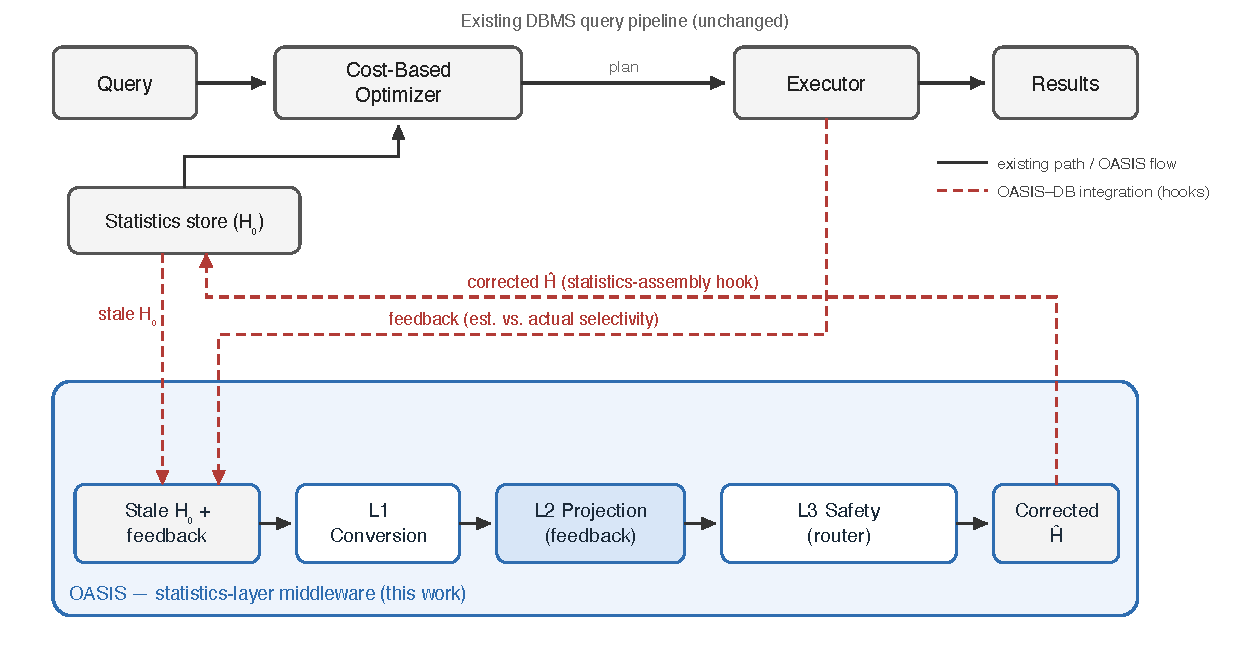
\includegraphics[width=\columnwidth]{figures/oasis_architecture.pdf}
  \caption{OASIS as a statistics-layer middleware. The existing DBMS query pipeline
  (solid, top) is left unchanged. OASIS runs its own input-to-correction flow (solid): it
  reads the stale histogram $H_0$ and a recent feedback window, then applies conversion
  (L1), feedback projection (L2), and safety routing (L3) to emit a corrected histogram $\hat H$. It
  attaches to the pipeline only through the dashed integration hooks---tapping predicate
  feedback from the executor and substituting $\hat H$ into the statistics the optimizer
  reads. All three layers are deterministic; L2 is the training-free feedback projection.}
  \label{fig:architecture}
\end{figure}

\emph{OASIS} names the approach---feedback-consistency repair guarded by a safety
router---and in its default deployed form applies the hard projection, with the residual-gated
Router (detailed in Section~\ref{sec:stage2}) as the fallback. The external baselines are the
stale histogram and ISOMER (the maximum-entropy projection initialized from stale), together
with the self-tuning histograms STHoles and QuickSel-H.

\subsection{Statistics-Format Conversion}
\label{sec:mcv-adapter}

Many engines do not expose a standalone editable equi-depth histogram. PostgreSQL,
for example, couples histogram boundaries with MCV lists and other per-column
summaries. We instantiate the interface for PostgreSQL-style statistics with a
three-phase adapter: reconstruct a canonical distribution view from the native
object, apply correction on the canonical view, and decompose the corrected view
back into native fields. The round trip preserves total mass to machine precision
(residual-quantile MAE mean $2.4\times10^{-17}$, max $9.2\times10^{-17}$), keeps
selectivity estimates consistent (global MAE $1.1\times10^{-4}$, worst case below
$0.39\%$), and completes in $0.066$--$0.073$\,ms.

Only the conversion layer is engine-specific; the projection and routing layers
operate on the canonical CDF and are unchanged across systems. Porting OASIS to a new
engine therefore reduces to writing one adapter. The effort depends on how the engine
exposes single-column statistics. MySQL and MariaDB keep equi-height/equi-width histograms
in the data dictionary and expose them through \texttt{ANALYZE TABLE \ldots\ UPDATE
HISTOGRAM} and \texttt{information\_schema}, which maps to the canonical CDF almost
directly. Microsoft SQL Server stores step-based histograms readable via
\texttt{DBCC SHOW\_STATISTICS}, again a close fit. Oracle couples height-balanced and
hybrid histograms with column-level density and is closest to the PostgreSQL case we
implement, where the adapter must also reconcile a most-common-value list. Engines that do
not expose an editable histogram object would require correcting statistics through their
maintenance API rather than in place. We validate the PostgreSQL adapter end-to-end; the
others are design targets, not claims, but they share the same canonical interface.

\subsection{The Repair Layer: Feedback Projection and the Router}
\label{sec:stage2}

The repair layer projects an input histogram onto the active feedback so
the result is consistent with what the executor observed, and a light router guards the
deployed correction. The same operator serves the single marginal and, in two dimensions, the
cross-column joint (Section~\ref{sec:crosscol}).

The hard operator is the ISOMER/IPF feedback-consistency
projection~\cite{markl2007consistent}: it builds the interval partition induced by the active
feedback predicates, initializes cell masses from the input histogram (the stale marginal, or
the independence grid for a joint), and performs cyclic I-projections until every active
predicate's interval mass matches its observed selectivity. When sequential drift makes the
active set inconsistent, the oldest constraints are dropped first. The operator is not new;
its role here is to realize the picture of Section~\ref{sec:problem}---it pins the statistic
exactly on the feedback span and leaves the maximum-entropy default elsewhere---and to provide
the safe form for joins and the planner.

On future single-column predicates, matching a handful of recent intervals exactly can
overfit; a soft operator that minimizes
$\mathrm{KL}(p\,\|\,p_{\text{prior}}) + \lambda \sum_j w_j (A_j p - y_j)^2$ over the same
partition generalizes slightly better, with $w_j=\exp(-(\text{conflict}_j/\tau)^2)$
down-weighting feedback the most recent observations contradict. We keep it as a router
candidate but do not build on it.

For robustness the deployed system can route among candidates---stale, the hard projection
(ISOMER), and the soft projection---selecting, per case, the one with the lowest
\emph{in-window feedback residual}: the mean absolute discrepancy, over the full recent
observation window, between a candidate's estimate and the observed selectivity. The gate
never observes test predicates, true cardinalities, runtimes, or plan shapes, and because the
pool contains the hard projection it can only lower the in-window residual. It is a fallback
that reverts to the maximum-entropy projection when a candidate over-extrapolates, not a
plan-shape guarantee; a plan-shape-aware gate is left to future work
(Section~\ref{sec:limitations}). On the planner configurations it selects ISOMER throughout
(Section~\ref{sec:postgres-planner}).

\section{Identifiability: When Feedback Pins the Statistic}
\label{sec:mechanism}

Section~\ref{sec:problem} framed feedback repair as constraining a distribution the
observations leave only partly determined. This section makes the \emph{identifiability}
question precise: when does query feedback pin the optimizer-relevant statistic, and when
does it leave a free part that no feedback-consistent method can resolve from feedback alone?
We answer with a rank condition and quantify how the free dimension shrinks as feedback
accumulates.

We now state the pinned regime precisely.

\begin{proposition}[Pinned regime]
\label{prop:pinned}
Adopt the cell-mass representation of Section~\ref{sec:problem}: the histogram grid and the
distinct active feedback endpoints partition the domain into $C$ cells, the marginal is the
cell-mass vector $m\in\Delta=\{m\in\mathbb{R}^{C}:m\ge 0,\ \mathbf{1}^\top m=1\}$ with
$\dim\Delta=C-1$, and the active feedback is \emph{consistent and noise-free}, written
$Am=y$ with $A\in\mathbb{R}^{K'\times C}$ and $r=\operatorname{rank}(A)$, the normalization
$\mathbf{1}^\top m=1$ being independent of the rows of $A$. Let $\Pi$ be the $I$-projection
onto the feasible set $F=\{m\in\Delta:Am=y\}$, applied identically to every method's prior,
and let $N=\ker A\cap\ker\mathbf{1}^\top$, so $\dim N=(C-1)-r$. Then:
\begin{enumerate}
  \item for any two priors $p,p'$ the projected marginals satisfy $\Pi(p)-\Pi(p')\in N$,
        so two priors can differ in their projected output \emph{only} on the
        $((C-1)-r)$-dimensional free subspace $N$; and
  \item if $r=C-1$ (the feedback identifies the marginal in this representation) then
        $N=\{0\}$ and $F$ is a single point, so $\Pi(p)=\Pi(p')$ for \emph{every} pair of
        priors. In particular the projections of the stale histogram (ISOMER) and of any
        other prior return the identical marginal.
\end{enumerate}
\end{proposition}

\begin{proof}[Proof sketch]
The $I$-projection onto a nonempty closed convex set returns a point of that set, so
$\Pi(p),\Pi(p')\in F$ and both satisfy $Am=y$ and $\mathbf{1}^\top m=1$. Their difference
$d=\Pi(p)-\Pi(p')$ therefore obeys $Ad=0$ and $\mathbf{1}^\top d=0$, i.e.\ $d\in N$, which
proves~(i). For the dimension, $N$ is the intersection of $\ker A$ (codimension $r$) with
the normalization hyperplane $\ker\mathbf{1}^\top$ (codimension $1$), and the two are
independent by assumption, so $\dim N=C-1-r$. When $r=C-1$ we get $\dim N=0$; the feasible
set $F$ is nonempty by consistency, hence a single point onto which every prior projects,
which proves~(ii).
\end{proof}

Two qualifications fix the scope of Proposition~\ref{prop:pinned}. First, the coincidence
in~(ii) concerns \emph{any prior closed by the same projection} $\Pi$, not the native
STHoles or QuickSel-H algorithms, which need not reduce to this $I$-projection; our
evaluation makes the comparison like-for-like by applying the same operator to every prior
(Section~\ref{sec:projection-init}), the setting in which the coincidence holds. Second, the
rank $r$ above is the \emph{exact} cell-level $\operatorname{rank}(A)$, whereas
Table~\ref{tab:mr_rank} reports an \emph{operational} rank on the $B-1$ exposed histogram
boundaries (Section~\ref{sec:problem})---a deployable proxy for $r$, not $r$ itself.

The Proposition is an \emph{identifiability} statement: when the feedback is rank-deficient
($r<C-1$) a free part $N$ remains, and \emph{no} feedback-consistent method can resolve it
from feedback alone---every such method must commit to some default there. ISOMER commits to
maximum entropy~\cite{markl2007consistent}, the least-committed choice; STHoles and
QuickSel-H commit to their own structural assumptions. Whether \emph{anything} can beat the
maximum-entropy default inside $N$ is then an empirical question, and the answer depends
sharply on dimension: for a single column it cannot
(Section~\ref{sec:single-column-results}), whereas for the cross-column joint it can, because
conjunctive feedback supplies the joint information the single-column free part never sees
(Section~\ref{sec:crosscol}).

We now make this prediction quantitative, since it governs how every later result should be
read. An equi-depth
marginal with $B{=}10$ buckets exposes $B-1=9$ free interior boundaries. For each held-out
case we count the independent feedback constraints (distinct interior boundary
anchors, merged within tolerance) and the residual free degrees of freedom (DOF).
Table~\ref{tab:mr_rank} reports the mean rank and free DOF as a function of the
feedback budget $K$.

\begin{table}[t]
  \centering\small
  \caption{Feedback-constraint rank and residual free degrees of freedom (DOF) of the
  marginal versus feedback budget $K$. We report an \emph{operational} rank on the
  $B{-}1=9$ exposed histogram boundaries---a deployable proxy for the exact cell-level
  $\mathrm{rank}(A)$ (Section~\ref{sec:problem}). Free DOF is the free-subspace dimension the
  projection leaves for the prior to complete; once feedback saturates the DOF the
  marginal is pinned and every method applying the same projection coincides
  (the pinned regime).}
  \label{tab:mr_rank}
  \setlength{\tabcolsep}{8pt}
  \begin{tabular}{r rr r}
    \toprule
    $K$ & mean rank & mean free DOF & marginals pinned \\
    \midrule
    2  & 2.32 & 6.68 & 0\% \\
    4  & 4.65 & 4.35 & 0\% \\
    6  & 6.95 & 2.05 & 6\% \\
    8  & 8.71 & 0.29 & 73\% \\
    12 & 8.98 & 0.02 & 98\% \\
    16 & 8.98 & 0.02 & 98\% \\
    \bottomrule
  \end{tabular}
\end{table}

The free DOF collapses from $6.68$ at $K{=}2$ to $\approx 0$ once the feedback
constraints saturate the $B-1$ boundaries---here by $K{\geq}12$ on this
constraint-spanning predicate population, with $73\%$ of marginals already pinned at
$K{=}8$. The free part is therefore a property of \emph{which regions of the domain the
feedback constrains}, not merely of how many observations there are: a finite window pins
the marginal near the observed predicates and leaves it free elsewhere. Two consequences
follow. (i) \emph{At saturation} the marginal is pinned and projection-based methods coincide
(Proposition~\ref{prop:pinned}); the dense PostgreSQL planner regime
(Section~\ref{sec:postgres-planner}) is exactly this tie. (ii) \emph{Below saturation} a free
part remains, but---as Section~\ref{sec:single-column-results} shows on real data---for a
single column the maximum-entropy default already fills it near-optimally, so the residual
free dimension is not an opportunity any prior can exploit. The exploitable structure
lies one level up, in the cross-column joint (Section~\ref{sec:crosscol}).

\section{Experimental Methodology}
\label{sec:experiments}

Our evaluation follows a maintained statistic along its deployment path, asking at each level
the one question that level can answer. We first establish the \emph{single-column} object on
real data: feedback projection repairs the stale marginal, and the maximum-entropy completion
is near-optimal---a learned prior and the self-tuning histograms give no edge
(Section~\ref{sec:single-column-results}). We then move one level up, to the \emph{cross-column}
joint, where feedback repairs the independence assumption that per-column statistics
structurally cannot (Section~\ref{sec:crosscol}). Finally we hand the corrected statistics to
real downstream consumers---composition estimators, a join kernel, and a live PostgreSQL
planner---and ask whether they stay safe (Section~\ref{sec:optimizer-facing}). The evaluation
is deliberately \emph{planner-facing}: we report the corrected statistics object together with
the row estimates and plan shapes a real optimizer derives from it, and use runtime only as a
single narrow TPC-H reality check that calibrated statistics track fresh-statistics behavior,
not as a claim of wall-clock superiority over stale statistics.

Unless stated otherwise, every feedback-driven method consumes the same observation budget
$K{=}16$ and emits corrected quantiles on the same $B{=}10$ grid; where a drift intensity $q$
is reported (Sections~\ref{sec:composition-family}, \ref{sec:factorjoin}) it scales how far
the post-drift distribution moves from the snapshot. The baselines fall into three classes:
(i) \emph{true self-tuning histograms}---STHoles~\cite{bruno2001stholes} and
ISOMER~\cite{markl2007consistent}, run as their published feedback-driven algorithms;
(ii) an \emph{adapted histogram-interface baseline}, QuickSel-H~\cite{park2020quicksel},
exposing QuickSel's density estimate on the shared grid (a faithful interface adaptation, not a
line-by-line reproduction); and (iii) an \emph{internal learned query-driven control}, LQM, a
monotone sigmoid-basis network fit online to the same feedback window, in the style of learned
query-driven estimators~\cite{kipf2019learned,li2023alece} but restricted to single-column
repair with the same no-rescan inputs. QuickSel-H and LQM are matched-interface stand-ins, not
the published systems---they calibrate where a flexible feedback-only fit lands relative to the
projection, and we draw no general claim against learned cardinality estimators. In the result
tables the \emph{OASIS} column is the deployed feedback projection, \emph{Unproj.\ prior} the
same correction \emph{without} that projection (a control), and the residual-gated selector
appears as \emph{Hybrid} or \emph{Router} (the same selector).

Every method starts from the \emph{same} stale
statistics, sees the \emph{same} feedback window, is projected onto the \emph{same}
constraints, and is evaluated on the \emph{same} held-out split; no method receives
oracle access, and ``fresh'' is computed from the post-drift data only as an accuracy
upper bound. Table~\ref{tab:metrics} defines the metrics used throughout.

\begin{table}[t]
  \centering\small
  \caption{Evaluation metrics. Direction marks whether lower ($\downarrow$), higher
  ($\uparrow$), or near-one ($\to 1$) is better. $\hat s,s^\ast$ are estimated and actual
  selectivity; $p$ is the corrected marginal; $A_j p$ is its mass on feedback interval
  $j$ with observed value $y_j$.}
  \label{tab:metrics}
  \setlength{\tabcolsep}{5pt}
  \begin{tabular}{l l c}
    \toprule
    Metric & Definition & Dir. \\
    \midrule
    Q-error & $\max(\hat s/s^\ast,\, s^\ast/\hat s)$, Eq.~\eqref{eq:qerr} & $\downarrow$ \\
    Selectivity MAE & mean $|\hat s - s^\ast|$ over predicates & $\downarrow$ \\
    Quantile MAE & mean $|v_i - v_i^{\text{fresh}}|$ over boundaries & $\downarrow$ \\
    Feedback residual & mean $|A_j p - y_j|$ on the observation window & $\downarrow$ \\
    Row Q-error & Q-error of \texttt{EXPLAIN} estimated rows vs \texttt{COUNT(*)} & $\downarrow$ \\
    Fresh-plan match & frac.\ of queries whose plan equals the fresh-stats plan & $\uparrow$ \\
    Recovery & frac.\ of stale/fresh plan disagreements the method fixes & $\uparrow$ \\
    New deviations & frac.\ of stale/fresh agreements the method breaks & $\downarrow$ \\
    Join regret & selected-plan proxy cost $/$ optimal proxy cost & $\downarrow$ \\
    Time/Fresh & geomean warm-cache runtime ratio to fresh stats & $\to 1$ \\
    \bottomrule
  \end{tabular}
\end{table}

\paragraph{Drift model and its justification}
We do not have access to a production stream of statistics-refresh histories, so we drive
staleness with controlled drift, chosen to mimic how analytical tables actually evolve
between \texttt{ANALYZE} passes. The drift intensity $q$ scales how far the post-drift
distribution moves from the snapshot $H_0$ (in units of inter-quantile shift), so larger
$q$ corresponds to a longer or more turbulent refresh interval; we sweep
$q\in\{1,\dots,30\}$ to cover mild to severe staleness. The drift \emph{families}
(batch loads, range and date-band shifts, skew evolution, outlier bursts, multimodal and
seasonal mixtures) are the update patterns that workload-evolution and learned-estimator
drift studies report as the practical causes of estimator degradation
\cite{li2022warper,negi2023robust,lee2023impact,han2024bytecard}. We treat the drift model
as a stated, transparent assumption rather than a claim about any single production system.

\section{Empirical Evaluation}
\label{sec:evaluation}

\subsection{Single-Column Repair: the Projection Is Near-Optimal on Real Data}
\label{sec:single-column-results}
\label{sec:projection-init}

The decisive single-column test is on real data. We draw individual columns from three
standard datasets (Power, Forest/Covtype, Census), drive drift with a sliding window over the
column in file order, and repair each column from a feedback window of $K$ observations. The
learned prior is trained \emph{only} on a disjoint pool of real columns (Wine Quality, Bike
Sharing) and never sees the test datasets. Every method initializes the \emph{same} feedback
projection; all are scored on held-out future predicates.

\begin{table}[t]
  \centering\small
  \caption{Single-column repair on held-out \emph{real} datasets (Power, Forest,
  Census), reusing the prior trained only on a disjoint pool of real columns. Stale is
  the uncorrected histogram; ISOMER is the maximum-entropy feedback projection; STHoles
  and QuickSel-H are self-tuning histograms; the learned prior is reported routed. All
  feedback methods cluster tightly and the learned prior gives \emph{no} gain over the
  max-entropy projection: on real single-column data, feedback projection is already
  near-optimal. Geometric-mean future-predicate Q-error ($\downarrow$).}
  \label{tab:real_singlecol}
  \setlength{\tabcolsep}{6pt}
  \begin{tabular}{l c r r r r r}
    \toprule
    Dataset & $K$ & Stale & ISOMER & STHoles & QuickSel-H & Learned \\
    \midrule
    Power & 16 & 1.511 & 1.182 & 1.171 & 1.245 & 1.164 \\
     & 2 & 1.528 & 1.362 & 1.356 & 1.408 & 1.346 \\
    \addlinespace[2pt]
    Forest & 16 & 1.766 & 1.125 & 1.113 & 1.104 & 1.104 \\
     & 2 & 1.813 & 1.472 & 1.464 & 1.470 & 1.451 \\
    \addlinespace[2pt]
    Census & 16 & 1.038 & 1.020 & 1.030 & 1.030 & 1.020 \\
     & 2 & 1.040 & 1.039 & 1.050 & 1.066 & 1.041 \\
    \addlinespace[2pt]
    \bottomrule
  \end{tabular}
\end{table}


Two things stand out in Table~\ref{tab:real_singlecol}. First, feedback repair works: the
maximum-entropy projection (ISOMER) cuts stale Q-error sharply---Forest from $1.77$ to
$1.13$, Power from $1.51$ to $1.18$---confirming that query feedback maintains a single-column
statistic well with no table rescan. Second, and central to this paper's design, \emph{no
method beats the projection}: STHoles, QuickSel-H, and the learned prior all land within
$1$--$2\%$ of ISOMER, at both dense ($K{=}16$) and sparse ($K{=}2$) feedback. The
maximum-entropy completion is already near-optimal for a single column, exactly as the
identifiability analysis (Section~\ref{sec:mechanism}) leads one to expect: the free part a
single column leaves is small and carries little structure a learned model can exploit beyond
the least-committed default. \emph{Single-column repair therefore needs no machine learning};
we adopt the training-free projection and turn, in Section~\ref{sec:crosscol}, to the
cross-column setting where feedback genuinely helps.

\subsection{Repairing the Independence Assumption from Feedback}
\label{sec:crosscol}

Single-column repair is the \emph{easy} regime: once the feedback projection is applied, the
maximum-entropy completion is near-optimal and a learned prior adds nothing
(Section~\ref{sec:single-column-results}). The optimizer's larger error is structural---the
attribute-value-independence (AVI) assumption, under which a conjunction's selectivity is the
product of the per-column selectivities. For correlated columns this is wrong no matter how
accurate each marginal is~\cite{poosala1997selectivity,leis2015good}, and no amount of
single-column repair can fix it. Query feedback, however, observes exactly the quantity AVI
gets wrong: the executor returns the true selectivity of a \emph{conjunctive} predicate.

We test whether conjunctive feedback can repair the joint. For a pair of columns we form the
true joint on a $G\times G$ grid ($G{=}12$); the AVI baseline is the outer product of the
\emph{true} marginals---the best case for independence, which isolates the correlation error
from any marginal error. The feedback estimate is a two-dimensional max-entropy (IPF)
projection that starts from the AVI grid and rescales it to match $K{=}16$ observed
conjunctive rectangle masses---the natural two-dimensional analogue of the single-column
ISOMER projection. Both are scored on held-out conjunctive rectangle predicates by
geometric-mean Q-error. We use eight real correlated column pairs drawn from the same public
datasets as the rest of the evaluation (Wine Quality, Bike Sharing, Forest/Covtype, Census,
Power), spanning weak to strong correlation.

\begin{table}[t]
  \centering\small
  \caption{Feedback-driven joint repair versus the independence assumption (AVI) on real
  correlated column pairs. AVI uses the true marginals (best case for independence); the
  feedback estimate is a 2D max-entropy (IPF) projection onto $K{=}16$ observed conjunctive
  rectangle masses. Geometric-mean conjunctive-predicate Q-error on held-out predicates;
  the gain over AVI is concentrated on the correlated pairs (negligible at $r{\approx}0$).}
  \label{tab:crosscol_feedback}
  \setlength{\tabcolsep}{6pt}
  \begin{tabular}{l r r r r}
    \toprule
    Real column pair & Pearson $r$ & AVI & Feedback & Improv. \\
    \midrule
    \texttt{census:age/hours} & $+0.07$ & 1.186 & 1.140 & $+3.9\%$ \\
    \texttt{forest:elev/roadway} & $+0.37$ & 1.326 & 1.237 & $+6.8\%$ \\
    \texttt{wred:density/alcohol} & $-0.50$ & 1.419 & 1.264 & $+10.9\%$ \\
    \texttt{wwhite:freeSO2/totSO2} & $+0.62$ & 1.491 & 1.312 & $+12.0\%$ \\
    \texttt{wred:fixedAcid/pH} & $-0.68$ & 1.532 & 1.358 & $+11.3\%$ \\
    \texttt{bike:casual/cnt} & $+0.69$ & 2.088 & 1.436 & $+31.2\%$ \\
    \texttt{forest:hill9/hill3} & $-0.78$ & 1.822 & 1.475 & $+19.1\%$ \\
    \texttt{bike:temp/atemp} & $+0.99$ & 1.688 & 1.492 & $+11.6\%$ \\
    \midrule
    \textbf{Aggregate} & & 1.538 & 1.328 & $+13.6\%$ \\
    \bottomrule
  \end{tabular}
\end{table}


Table~\ref{tab:crosscol_feedback} reports the result, and it follows the structure the
analysis predicts. Where the columns are essentially independent (Census \texttt{age}/\texttt{hours},
$r{=}0.07$) feedback repair barely moves the estimate ($+3.9\%$): there is no correlation to
recover and AVI is already right. Where the columns are correlated, feedback repair wins
decisively---from $+7\%$ to $+31\%$ across the correlated pairs, largest on the strongly
dependent \texttt{casual}/\texttt{cnt} pair, for a $13.6\%$ aggregate reduction in conjunctive
Q-error over AVI. The gain follows the \emph{presence} of correlation---vanishing as columns
approach independence---rather than scaling strictly with $|r|$. Unlike the single-column
case, the cross-column information that independence discards is large and
\emph{feedback-fillable}: conjunctive observations carry exactly the joint mass per-column
statistics structurally lack. This is where feedback maintenance earns its keep for the
optimizer---and, as in the single-column case, the repair operator is the training-free
max-entropy projection, now in two dimensions.

\paragraph{Validation on the Join Order Benchmark}
The pairs above use real columns but a controlled predicate suite. We therefore repeat the
test on the Join Order Benchmark (JOB), the standard real-data cardinality-estimation
benchmark, querying its IMDB tables inside a live PostgreSQL~14 planner. For correlated
column pairs we score the geometric-mean Q-error of conjunctive predicates (range on numeric
columns, equality on categorical ones) under four estimators: PostgreSQL's default
(per-column statistics plus independence); PostgreSQL's own multi-column \emph{extended}
statistics (\texttt{CREATE STATISTICS}, built from a full scan); independence with the
\emph{true} marginals (\textsc{avi}, which isolates the cross-column error from per-column
error); and the OASIS feedback-repaired joint ($K{=}16$ observed conjunctive masses, no scan).

\begin{table}[t]
  \centering\small
  \caption{Cross-column repair on the Join Order Benchmark (real IMDB tables, live
  PostgreSQL~14). Geometric-mean conjunctive-predicate Q-error ($\downarrow$) for
  PostgreSQL-default (per-column $+$ independence), PostgreSQL extended statistics
  (\texttt{CREATE STATISTICS}, scan-built), independence with true marginals (\textsc{avi}),
  and the OASIS feedback-repaired joint (no scan). The conservative cross-column effect is
  \textsc{avi}$\to$OASIS; \texttt{person\_info} is a near-independent control.}
  \label{tab:crosscol_job}
  \setlength{\tabcolsep}{5pt}
  \begin{tabular}{l r r r r r}
    \toprule
    Real IMDB column pair & $r$ & PG-def. & PG-ext. & \textsc{avi} & OASIS \\
    \midrule
    \texttt{title.prod\_year/kind}        & $0.35$  & $5.69$ & $5.63$ & $5.70$ & $\mathbf{1.95}$ \\
    \texttt{aka\_title.prod\_year/kind}   & $0.29$  & $3.85$ & $3.93$ & $3.75$ & $\mathbf{1.67}$ \\
    \texttt{cast\_info.nr\_order/role}    & $0.01$  & $78.2$ & $77.6$ & $2.27$ & $\mathbf{1.63}$ \\
    \texttt{movie\_comp.ctype/cid}        & $0.51$  & $62.4$ & $62.3$ & $1.25$ & $\mathbf{1.09}$ \\
    \texttt{title.season/episode}         & $-0.02$ & $37.7$ & $39.4$ & $1.51$ & $\mathbf{1.45}$ \\
    \texttt{person\_info.itype/pid}~(ctrl)& $0.04$  & $58.9$ & $58.9$ & $1.08$ & $1.09$ \\
    \bottomrule
  \end{tabular}
\end{table}

Table~\ref{tab:crosscol_job} shows three things. First, where the optimizer's error is
genuinely the independence assumption---\texttt{production\_year}$\times$\texttt{kind\_id} in
\texttt{title} and \texttt{aka\_title}, where PostgreSQL's default already matches the
true-marginal \textsc{avi} baseline---feedback joint repair cuts conjunctive Q-error by
$56$--$66\%$. Second, on a near-independent control (\texttt{person\_info}, an identifier
column) it has no effect ($-1\%$), confirming the repair is specific to genuine dependence.
Third, PostgreSQL's conjunctive estimates on these columns are badly off (up to $78\times$),
and its own extended statistics do \emph{not} help---their MCV/dependency machinery covers
common combinations, not the correlated tail---whereas the feedback-repaired joint brings the
error to $1.1$--$2.0\times$. Where PostgreSQL's error far exceeds the true-marginal baseline
(e.g.\ \texttt{cast\_info}, $78\times$ versus $2.3\times$), most of that gap is PostgreSQL's
\emph{per-column} estimation error on skewed columns rather than independence; we therefore
report the conservative cross-column effect as the \textsc{avi}$\to$OASIS reduction, which is
feedback repair alone.

\subsection{From Better Estimates to Better Plans: a JOB Case Study}
\label{sec:plan-level}
Lower conjunctive Q-error is only useful if it changes what the optimizer \emph{does}. We
therefore ask, directly on JOB, whether a feedback-repaired cross-column estimate can flip a
join order and improve end-to-end runtime. Because JOB is a static benchmark, there is no
``re-scan'' baseline; the natural reference is the \emph{oracle} plan obtained by injecting the
\emph{true} cardinality, which upper-bounds what any repair could achieve. For each candidate
query we locate the correlated sub-expression, compute PostgreSQL's estimate, OASIS's repaired
estimate ($K{=}16$ feedback, no scan), and the true count, and inject each as a single
\texttt{Rows} hint via \texttt{pg\_hint\_plan}, then measure the warm-cache plan and runtime.
This is a \emph{targeted case study}, not a runtime benchmark: we report where the mechanism
reaches end-to-end and, just as deliberately, where it does not.

\begin{table}[t]
  \centering\small
  \caption{Plan-level injection on JOB (live PostgreSQL~14, warm cache). Each row injects the
  corrected local conjunctive cardinality as a \texttt{Rows} hint. ``Local Q-err'' is the
  estimate for the correlated sub-expression (PG\,$\to$\,OASIS); runtimes are
  default\,/\,OASIS\,/\,oracle (oracle injects the true count).}
  \label{tab:plan_level_job}
  \setlength{\tabcolsep}{5pt}
  \begin{tabular}{l r r r r}
    \toprule
    Query & Local Q-err & default & OASIS & oracle \\
          & (PG$\to$OASIS) & (ms) & (ms) & (ms) \\
    \midrule
    \texttt{q00964} (\texttt{prod\_year}$\times$\texttt{kind}) & $61.1\to3.5$ & $1952$ & $\mathbf{25.5}$ & $22.5$ \\
    \texttt{q00508} (empty-result case)                        & $3.3{\cdot}10^{13}\to1.0$ & $3443$ & $\mathbf{2877}$ & $2877$ \\
    \bottomrule
  \end{tabular}
\end{table}

The headline case is exactly the correlation behind Table~\ref{tab:crosscol_job}:
\texttt{title.production\_year}$\times$\texttt{kind} (query \texttt{q00964},
\texttt{production\_year}${}>{}$\texttt{2014} \textsc{and} \texttt{kind}${}={}$\texttt{movie}).
PostgreSQL estimates the correlated branch at $7$ rows against a true $428$ ($61\times$ under);
the feedback joint repairs it to $122$ ($3.5\times$), which is enough to change the join order.
The resulting plan runs in $25.5$\,ms versus PostgreSQL's $1952$\,ms---a $76.7\times$
speedup---and essentially matches the oracle plan's $22.5$\,ms (Table~\ref{tab:plan_level_job}).
A second case (\texttt{q00508}) is an empty-result query that PostgreSQL mis-estimates at
$3.3{\cdot}10^{13}$; the repair collapses it to the correct near-zero estimate for a smaller
$1.2\times$ gain.

We are equally explicit about the boundary. Across the broader sweep, OASIS's repair acts on the
\emph{local} conjunctive selectivity, but several plan-critical errors live at a \emph{downstream
join} cardinality that the local fix does not propagate to: in five queries the oracle hint flips
the plan for a $6$--$8.8\times$ speedup while the OASIS-corrected local estimate does not reach
the flip, and in one query the corrected estimate steered PostgreSQL to a slightly worse plan
($2.1\times$ slower). The canonical $113$-query JOB sweep produced no plan changes at all. The
honest reading is that feedback repair of cross-column statistics \emph{can} produce large,
oracle-matching end-to-end gains when the dependence error sits on a join-order-critical base
predicate, and that closing the residual gap requires propagating repair to intermediate join
cardinalities---which our base-table statistics layer does not yet do (Section~\ref{sec:limitations}).

\subsection{Downstream Optimizer Consumption}
\label{sec:optimizer-facing}

A corrected single-column statistic is only as good as what its consumers can safely do with
it. This section tests a single claim---\emph{a feedback-consistent (projected) statistic is
safe for any consumer, whereas an unprojected correction can be useless or actively
harmful}---and tests it along an escalating axis rather than re-establishing it four times.
Each rung adds exactly one thing the previous cannot: six composition estimators show the claim
is \emph{consumer-agnostic} (Section~\ref{sec:composition-family}); a bilinear FactorJoin kernel
is the \emph{nonlinear stress case}, where an unprojected correction turns harmful
(Section~\ref{sec:factorjoin}); a live PostgreSQL planner is the \emph{real-system} test on row
estimates and plan shapes (Section~\ref{sec:postgres-planner}); and TPC-H is the lone
\emph{runtime} reality check (Section~\ref{sec:tpch-runtime}). Because the OASIS and
\emph{Unproj.\ prior} columns differ only in the projection, every rung also isolates how much
of the benefit is the projection rather than the prior. The primary evidence is estimate quality and
plan \emph{shape}; runtime enters only in the final, deliberately narrow check.

\subsubsection{Composition-Family Generalization}
\label{sec:composition-family}

We embed OASIS as a drop-in marginal source in six independently designed composition
estimators---the independence/maximum-entropy estimator, IPF/Sinkhorn on a 2D grid,
and Gaussian, Clayton, Gumbel, and Frank copulas---varying only the marginal input.
The dependence structure is held fixed and identical for every marginal, so this is a
clean marginal ablation, and the Archimedean copulas are intentionally mis-specified
for the Gaussian-correlated data.

\begin{figure}[t]
  \centering
  \begin{subfigure}{\linewidth}
    \centering
    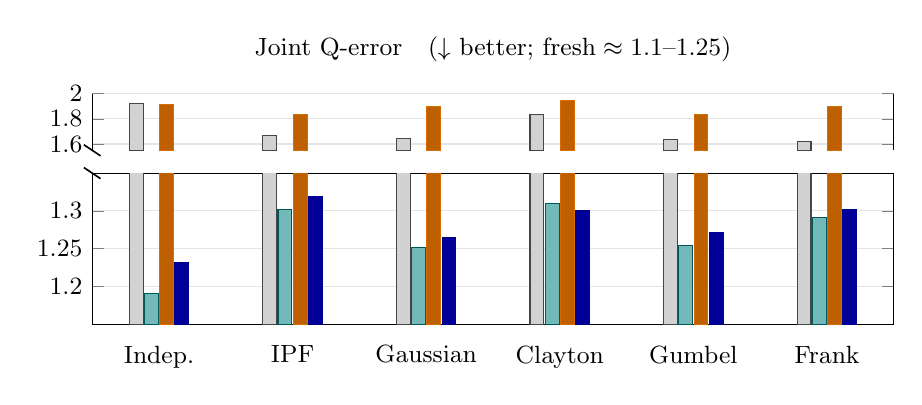
\begin{tikzpicture}
      \pgfplotsset{cmpstyle/.style={
          ybar=0.5pt, bar width=5pt, width=.97\columnwidth,
          symbolic x coords={Indep.,IPF,Gaussian,Clayton,Gumbel,Frank}, xtick=data,
          enlarge x limits=0.10, ymajorgrids, grid style={gray!20},
          tick label style={font=\small}, label style={font=\small}}}
      \begin{axis}[cmpstyle, name=cmup, height=2.3cm,
          ymin=1.55, ymax=2.0, ytick={1.6,1.8,2.0}, axis x line=none,
          title={\small Joint Q-error\quad($\downarrow$ better; fresh${}\approx{}1.1$--$1.25$)},
          title style={yshift=2pt},
        ]
        \addplot[fill=gray!35,draw=gray!55!black] coordinates {(Indep.,1.924)(IPF,1.668)(Gaussian,1.645)(Clayton,1.836)(Gumbel,1.639)(Frank,1.621)};
        \addplot[draw=none,fill=none] coordinates {(Indep.,1.191)(IPF,1.302)(Gaussian,1.251)(Clayton,1.310)(Gumbel,1.254)(Frank,1.291)};
        \addplot[fill=orange!75!black,draw=orange!85!black] coordinates {(Indep.,1.913)(IPF,1.837)(Gaussian,1.901)(Clayton,1.949)(Gumbel,1.833)(Frank,1.899)};
        \addplot[draw=none,fill=none] coordinates {(Indep.,1.231)(IPF,1.319)(Gaussian,1.265)(Clayton,1.300)(Gumbel,1.271)(Frank,1.302)};
      \end{axis}
      \begin{axis}[cmpstyle, name=cmlo, at={(cmup.below south west)}, anchor=north west, yshift=-1.5mm,
          height=3.5cm, ymin=1.15, ymax=1.35, ytick={1.2,1.25,1.3},
          xtick style={draw=none},
        ]
        \addplot[fill=gray!35,draw=gray!55!black] coordinates {(Indep.,1.924)(IPF,1.668)(Gaussian,1.645)(Clayton,1.836)(Gumbel,1.639)(Frank,1.621)};
        \addplot[fill=teal!55,draw=teal!70!black] coordinates {(Indep.,1.191)(IPF,1.302)(Gaussian,1.251)(Clayton,1.310)(Gumbel,1.254)(Frank,1.291)};
        \addplot[fill=orange!75!black,draw=orange!85!black] coordinates {(Indep.,1.913)(IPF,1.837)(Gaussian,1.901)(Clayton,1.949)(Gumbel,1.833)(Frank,1.899)};
        \addplot[fill=blue!60!black,draw=blue!55!black] coordinates {(Indep.,1.231)(IPF,1.319)(Gaussian,1.265)(Clayton,1.300)(Gumbel,1.271)(Frank,1.302)};
      \end{axis}
      \draw[draw=white,line width=2.2pt] (cmup.south west) -- (cmlo.north west);
      \draw[semithick] ($(cmup.south west)+(-3pt,2pt)$) -- ($(cmup.south west)+(3pt,-2pt)$);
      \draw[semithick] ($(cmlo.north west)+(-3pt,2pt)$) -- ($(cmlo.north west)+(3pt,-2pt)$);
    \end{tikzpicture}
    \caption{Composition family (six estimators; dependence fixed, only the marginal varies):
    the projection (ISOMER, and OASIS, which coincides with it) recovers most of the stale
    joint Q-error, whereas the unprojected prior stays near stale.}
    \label{fig:composition_family}
  \end{subfigure}

  \vspace{1mm}
  \begin{subfigure}{\linewidth}
    \centering
    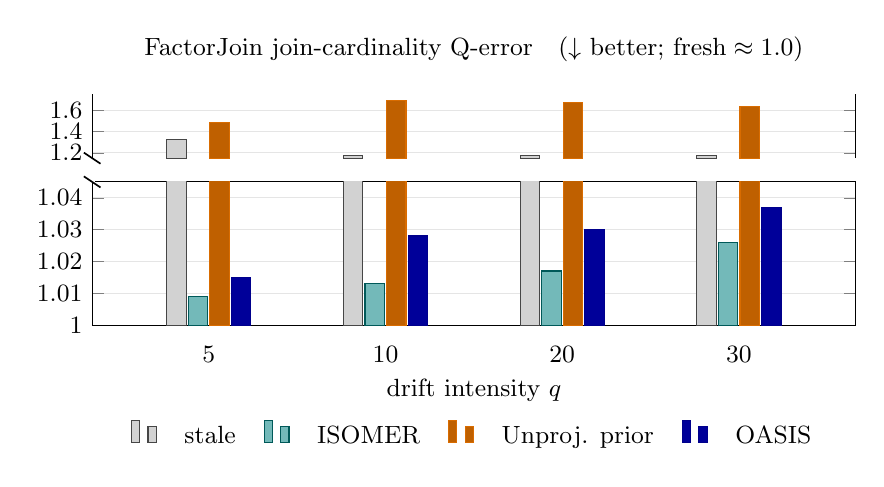
\begin{tikzpicture}
      \pgfplotsset{fjstyle/.style={
          ybar=0.8pt, bar width=7pt, width=.93\columnwidth,
          symbolic x coords={5,10,20,30}, xtick=data, enlarge x limits=0.22,
          ymajorgrids, grid style={gray!20},
          tick label style={font=\small}, label style={font=\small}}}
      \begin{axis}[fjstyle, name=fjup, height=2.4cm,
          ymin=1.15, ymax=1.76, ytick={1.2,1.4,1.6}, axis x line=none,
          title={\small FactorJoin join-cardinality Q-error\quad($\downarrow$ better; fresh${}\approx{}1.0$)},
          title style={yshift=2pt},
        ]
        \addplot[fill=gray!35,draw=gray!55!black] coordinates {(5,1.323)(10,1.179)(20,1.179)(30,1.178)};
        \addplot[draw=none,fill=none] coordinates {(5,1.009)(10,1.013)(20,1.017)(30,1.026)};
        \addplot[fill=orange!75!black,draw=orange!85!black] coordinates {(5,1.484)(10,1.699)(20,1.673)(30,1.638)};
        \addplot[draw=none,fill=none] coordinates {(5,1.015)(10,1.028)(20,1.030)(30,1.037)};
      \end{axis}
      \begin{axis}[fjstyle, name=fjlo, at={(fjup.below south west)}, anchor=north west, yshift=-1.5mm,
          height=3.4cm, ymin=1.0, ymax=1.045, ytick={1.00,1.01,1.02,1.03,1.04},
          xtick style={draw=none}, xlabel={drift intensity $q$}, xlabel style={yshift=1pt},
          legend style={at={(0.5,-0.62)}, anchor=north, legend columns=-1,
            font=\small, draw=none, column sep=8pt},
        ]
        \addplot[fill=gray!35,draw=gray!55!black] coordinates {(5,1.323)(10,1.179)(20,1.179)(30,1.178)};
        \addplot[fill=teal!55,draw=teal!70!black] coordinates {(5,1.009)(10,1.013)(20,1.017)(30,1.026)};
        \addplot[fill=orange!75!black,draw=orange!85!black] coordinates {(5,1.484)(10,1.699)(20,1.673)(30,1.638)};
        \addplot[fill=blue!60!black,draw=blue!55!black] coordinates {(5,1.015)(10,1.028)(20,1.030)(30,1.037)};
        \legend{stale, ISOMER, Unproj. prior, OASIS}
      \end{axis}
      \draw[draw=white,line width=2.2pt] (fjup.south west) -- (fjlo.north west);
      \draw[semithick] ($(fjup.south west)+(-3pt,2pt)$) -- ($(fjup.south west)+(3pt,-2pt)$);
      \draw[semithick] ($(fjlo.north west)+(-3pt,2pt)$) -- ($(fjlo.north west)+(3pt,-2pt)$);
    \end{tikzpicture}
    \caption{FactorJoin bin-based join kernel as the join-key distribution drifts (only the
    single-column key histogram varies). The unprojected prior is \emph{actively harmful}---its
    Q-error exceeds even stale, because the bilinear kernel amplifies mass-concentration
    errors---whereas the projected methods track the fresh marginal ($\approx 1.0$).}
    \label{fig:factorjoin}
  \end{subfigure}
  \caption{Downstream consumption of the maintained statistic. A feedback-consistent
  (\emph{projected}) statistic is safe for any consumer, whereas an \emph{unprojected} prior is
  not---weak or negative in the composition family (a), and actively harmful in the bilinear
  FactorJoin kernel (b). Each panel uses a broken axis (upper for the large values, lower
  zoomed on the recovered cluster): the feedback projection, not the prior, is what keeps the
  maintained statistic safe to consume.}
  \label{fig:downstream}
\end{figure}

Figure~\ref{fig:composition_family} shows the claim holds across all six estimators: the
feedback projection recovers $19.7\%$--$36.0\%$ of the stale joint Q-error, while an unprojected
correction yields weak or negative gains. The benefit is therefore \emph{consumer-agnostic}---it
does not depend on a single dependence model and survives even the intentionally mis-specified
Archimedean copulas.

\subsubsection{FactorJoin Integration}
\label{sec:factorjoin}

To test propagation into a learned \emph{join} estimator, we embed OASIS in the
bin-based join kernel of FactorJoin~\cite{wu2023factorjoin}. For an equi-join
$A.k=B.k$ it estimates
$\sum_{\text{bin}}\mathrm{cnt}_A[\text{bin}]\,\mathrm{cnt}_B[\text{bin}]/\mathrm{dv}[\text{bin}]$,
where each per-bin key frequency comes from a single-column key histogram, which we make
the OASIS-correctable object. The keys are generated independently, so only the
single-column key histogram varies across methods.

% FactorJoin result is now panel (b) of the two-panel Figure~\ref{fig:downstream} above.

Figure~\ref{fig:factorjoin} is the sharp case the escalation was built for. Because the kernel
is bilinear in per-bin mass, it amplifies mass-concentration errors, and the unprojected
correction becomes \emph{actively harmful}---aggregate join Q-error $1.621$, worse than the
stale $1.213$ it was meant to repair. Feedback projection reverses this: OASIS improves over
stale at every drift level ($+12.0\%$--$+23.2\%$, $+15.3\%$ aggregate; the Hybrid $+16.1\%$) and
tracks the fresh marginal throughout. A correction that helped the mild consumers above can
\emph{hurt} a nonlinear one unless it is first projected onto the feedback.

\subsubsection{PostgreSQL Planner-Only Statistics Injection}
\label{sec:postgres-planner}

We validate that corrected statistics affect a real optimizer pipeline. The experiment
builds alternative single-column statistics for \texttt{fact.x} and injects them into
\texttt{pg\_statistic}; true rows come from \texttt{COUNT(*)}, estimated rows and plan
shapes from \texttt{EXPLAIN (FORMAT JSON)}. No query runtime is measured. The batch
covers two drift directions, two table sizes, and three seeds (12 configurations).

\begingroup
\oasisUseMaxWidthResize{.88\columnwidth}
\begin{table}[t]
  \centering
  \small
  \caption{Multi-configuration PostgreSQL planner-only statistics-injection evidence. Values are means over configurations; parentheses show one standard deviation across configurations. True rows use \texttt{COUNT(*)}; estimated rows and plan shapes use \texttt{EXPLAIN (FORMAT JSON)}. No query runtime is measured.}
  \label{tab:postgres_planner_stats_injection_batch}
  \setlength{\tabcolsep}{3pt}
  \resizebox{\textwidth}{!}{%
  \begin{tabular}{lrrrr}
    \toprule
    Method & Row QE & Fresh Plan & Recovery & New Deviations \\
    \midrule
    Stale & 28.453 (6.576) & 56.1\% (5.1) & 0.0\% (0.0) & 0.0\% (0.0) \\
    ISOMER & 2.390 (0.286) & 96.0\% (1.9) & 91.9\% (3.9) & 1.0\% (1.0) \\
    OASIS-noProj & 3.894 (1.252) & 90.9\% (5.1) & 80.7\% (14.4) & 2.4\% (1.9) \\
    OASIS & 2.377 (0.269) & 95.9\% (1.9) & 91.7\% (3.8) & 1.0\% (1.0) \\
    Soft & 2.452 (0.312) & 96.0\% (1.9) & 91.9\% (3.9) & 1.0\% (1.0) \\
    Hybrid & 2.391 (0.289) & 96.0\% (1.9) & 91.9\% (3.9) & 1.0\% (1.0) \\
    Aggressive & 2.382 (0.283) & 96.0\% (1.9) & 91.9\% (3.9) & 1.0\% (1.0) \\
    Router & 2.386 (0.288) & 96.1\% (2.0) & 92.1\% (4.1) & 1.0\% (1.0) \\
    Fresh & 1.415 (0.092) & 100.0\% (0.0) & 100.0\% (0.0) & 0.0\% (0.0) \\
    \bottomrule
  \end{tabular}
  }
\end{table}

\endgroup

Table~\ref{tab:postgres_planner_stats_injection_batch} is the strongest DBMS-facing
evidence, and its claim is deliberately one of \emph{plan-shape safety}, not accuracy
superiority over ISOMER. Pooling over all query instances, stale statistics give
aggregate row Q-error $27.768$ and match the fresh plan on $56\%$ of queries.
(All numbers in this paragraph are pooled over query instances;
Table~\ref{tab:postgres_planner_stats_injection_batch} instead reports
the per-configuration mean$\pm$sd, which differs slightly---e.g.\ stale row Q-error is
$28.453$ averaged over configurations versus $27.768$ pooled.)
An unprojected correction reduces row Q-error to $3.703$ but introduces new plan deviations
in $2.3\%$ of cases. The feedback projection (OASIS) reduces row Q-error to $2.362$, matches the fresh plan on
$95.9\%$ of queries, recovers $92.1\%$ of stale/fresh disagreements, and cuts new
deviations to $1.1\%$. Crucially, OASIS ($2.362$) and ISOMER ($2.374$) are near-identical here---the rank mechanism,
not a disappointment: these planner-facing windows are dense enough to pin the active
constraints (Section~\ref{sec:mechanism}), so hard projection converges to nearly the same
marginal whichever prior seeds it, and the Router selects ISOMER on all twelve configurations.
On a real optimizer, then, feedback maintenance restores near-fresh plans with no table scan,
and the projection alone suffices.


\subsubsection{TPC-H DML-Drift Runtime Sanity Check}
\label{sec:tpch-runtime}

This runtime check states its claim up front: calibrated statistics \emph{reproduce
fresh-statistics behavior}---accuracy, plan shape, and runtime---rather than beat the stale
baseline on wall-clock. We load TPC-H
SF10, drift it with an RF1-style insert stream that shifts \texttt{lineitem.l\_shipdate}
and \texttt{orders.o\_orderdate} into a new date band, and inject single-column
statistics for those columns exactly as above, reusing the \emph{same} pretrained prior
with no TPC-H retraining (also a cross-schema generalization test). For six
date-sensitive queries we record scan row Q-error, plan shape, and warm-cache
\texttt{EXPLAIN ANALYZE} time over three refresh-stream seeds. Because warm-cache
runtime is determined by the induced plan, we time each distinct $(\text{query},
\text{plan})$ once at full repetition and assign it to every method sharing that plan.

\begingroup
\oasisUseMaxWidthResize{.92\columnwidth}
\begin{table}[t]
\centering
\small
\caption{TPC-H SF10 DML-drift study, aggregated over three independent refresh-stream seeds (mean\,$\pm$\,std; six curated date-sensitive queries each; planner-only statistics injection, PostgreSQL~14). The pretrained OASIS prior is reused with no TPC-H retraining. \emph{Scan Q-err} is the row-estimation error on the drifting date column. \emph{Time/Fresh} and \emph{Time/Stale} are geometric-mean ratios of warm-cache \texttt{EXPLAIN ANALYZE} execution time to the fresh- and stale-statistics runs. Calibrated statistics (OASIS, Router) track fresh statistics within the reported distribution (median Time/Fresh $\approx 1$, worst case $\le 1.40$) and induce no plan-shape deviation from fresh across the 18 query instances. The stale wall-clock baseline is not a reliable target: a stale mis-estimate can pick a coincidentally cheaper-to-run plan (Time/Stale $>1$ here), whereas in other configurations it picks a much slower one; we therefore make no runtime-superiority claim and report that OASIS reproduces fresh-statistics behavior.}
\label{tab:tpch_runtime}
\setlength{\tabcolsep}{5pt}
\begin{tabular}{lccc}
\toprule
Method & Scan Q-err & Time/Fresh & Time/Stale \\
\midrule
Stale & 5.23\,$\pm$\,0.24 & 0.65\,$\pm$\,0.07 & 1.00\,$\pm$\,0.00 \\
ISOMER & 2.02\,$\pm$\,0.08 & 0.98\,$\pm$\,0.07 & 1.51\,$\pm$\,0.07 \\
OASIS-noProj & 2.66\,$\pm$\,0.07 & 1.02\,$\pm$\,0.02 & 1.59\,$\pm$\,0.18 \\
OASIS & 2.02\,$\pm$\,0.10 & 0.96\,$\pm$\,0.04 & 1.49\,$\pm$\,0.11 \\
Router & 2.01\,$\pm$\,0.10 & 1.01\,$\pm$\,0.02 & 1.57\,$\pm$\,0.15 \\
Fresh & 2.01\,$\pm$\,0.07 & 1.00\,$\pm$\,0.00 & 1.56\,$\pm$\,0.17 \\
\bottomrule
\end{tabular}
\end{table}

\endgroup

Table~\ref{tab:tpch_runtime} reports the result. Accuracy is unambiguous: stale scan
Q-error $5.23\pm0.24$ is repaired to $2.02$ for OASIS and $2.01$ for the Router,
matching fresh ($2.01$), on a standard schema with no retraining. Calibrated statistics
track the \emph{fresh}-statistics runtime to within a few percent (time-to-fresh
$0.96$ for OASIS, $1.01$ for the Router) because they induce the fresh plans. The
\emph{stale} wall-clock baseline is not a reliable target: here the stale mis-estimate
happens to pick a cheaper-to-run plan, so calibrated and fresh statistics run
$\approx 1.5\times$ slower than stale---the price of the correct plan, paid equally by
fresh---whereas in a larger-drift configuration the same mis-estimate produced a plan
$1.56\times$ slower than fresh. The deployment-relevant invariant is that calibrated
statistics track fresh statistics in both accuracy and runtime, while stale statistics
make the wall-clock outcome unpredictable in either direction. This is a single-schema
check on six queries; we draw no broader runtime-superiority conclusion.

Because a median or geomean can hide a bad tail, we report the runtime distribution against
the deployment target, fresh statistics, over all 18 query instances (six queries, three
seeds). Calibrated statistics induce the fresh plan on every instance---\emph{zero} plan
deviations from fresh for OASIS, the Router, and ISOMER---so there is no plan-shape tail.
The runtime-to-fresh ratio stays tight: median $0.96$ and worst-case $1.23$ for OASIS,
median $1.00$ and worst-case $1.40$ for the Router. The only large ratio appears against
\emph{stale}, on the single query (TPC-H Q14) whose plan changes stale$\to$fresh: under
stale's coincidentally cheap plan it runs much faster---up to $\approx 13\times$ in the
worst instance---but fresh statistics show a comparable gap there, so this is the cost of
switching to the correct plan, not a regression introduced by calibration. No calibrated method is slower than fresh by more than
$1.4\times$ on any query or seed.

\subsection{Overhead and Deployment}
\label{sec:overhead}

A per-column correction is the feedback projection (a handful of I-projection sweeps over the
$B$ buckets) plus the PostgreSQL-style format conversion ($0.066$--$0.073$\,ms); it completes
in well under a millisecond and uses no learned model. Feedback collection adds bounded
per-conjunct bookkeeping, emitting one observation tuple per conjunct at query completion. A
correction therefore avoids the full-table \texttt{ANALYZE} scan a refresh would incur---the intended use case is
maintaining optimizer-facing statistics \emph{between} scheduled refreshes, not
replacing full refreshes after major schema changes or bulk shifts.

\section{Related Work}
\label{sec:related}

\paragraph{Feedback-driven statistics and the completion question}
Cost-based optimization and selectivity estimation rely on compact statistics built
from scans
\cite{selinger1979access,chaudhuri1998overview,ioannidis1993histogram,poosala1997selectivity},
with streaming summaries such as KLL sketches providing approximate
quantiles~\cite{ivkin2019kll} and query feedback long used to adapt
estimates~\cite{chen1994adaptive}. Self-tuning histograms, STHoles, SASH, and ISOMER
refine statistics from observed results
\cite{aboulnaga1999self,bruno2001stholes,lim2003sash,markl2007consistent}, and
execution-feedback frameworks repair optimizer state over
time~\cite{chaudhuri2008paygo}. OASIS shares this statistics-facing target but treats feedback
repair as an \emph{identifiability} problem---a rank condition for when feedback pins the
optimizer-relevant statistic (Proposition~\ref{prop:pinned})---and use it to separate two
regimes the prior literature does not distinguish: single-column repair, where the
maximum-entropy projection is near-optimal and learning is unnecessary, and cross-column
repair, where feedback corrects the independence assumption the per-column statistics
structurally cannot. The attribute-value-independence assumption and its cost are long
documented~\cite{poosala1997selectivity,leis2015good}; engines mitigate it with
multi-dimensional or extended statistics built from scans, and STHoles~\cite{bruno2001stholes}
builds multidimensional histograms from feedback. OASIS differs in maintaining both the
marginal and, for correlated columns, the joint from query feedback alone---no rescan, with a
safety router---and in characterizing when feedback suffices.

\paragraph{Learned cardinality estimation}
Learned estimators such as NeuroCard, Naru, DeepDB, FACE, MSCN, FLAT, and Iris predict
cardinalities from learned density or representation models
\cite{yang2020neurocard,yang2019deep,hilprecht2019deepdb,yang2020face,kipf2019learned,zhu2021flat,lu2022pretraining},
and benchmark and deployment studies document both their promise and the difficulty of
robustness across workloads and drift
\cite{wang2021ready,sun2021designspace,kim2022learnedstudy,han2021cardinality,li2022warper,negi2023robust,li2023alece,wang2023ceda,wang2023ldss,han2024bytecard}.
This line remains active in the database-systems literature: recent work learns dynamic sample selectors for
cardinality estimation~\cite{wang2023dynamicsample} and recursive-network models of complex
predicates~\cite{wang2024recursivepred}. These systems output point estimates or estimator
state; OASIS instead repairs the optimizer's own marginal \emph{statistics} from query feedback
for an existing CBO to consume unchanged, rather than replacing the estimator with a learned
model.

\paragraph{Composition, joins, and plan-level learning}
Copula and factorized-join estimators such as FactorJoin~\cite{wu2023factorjoin} combine
one-dimensional marginals with a dependence or join-key model; our composition-family and
FactorJoin experiments embed OASIS as the marginal source in exactly these estimators and
show feedback consistency is a prerequisite for safe downstream use. Plan-level and robust
optimization systems---mid-query re-optimization, progressive optimization, LEO, Neo, Bao,
and Flow-Loss
\cite{kabra1998efficient,markl2004progressive,babcock2005robust,stillger2001leo,marcus2019neo,marcus2022bao,negi2021flowloss,lee2023impact}---adjust
plan choices or train plan-relevant estimates; OASIS operates below them by correcting the
statistics object itself, and the two are complementary.

\section{Limitations}
\label{sec:limitations}

The most important boundary is external validity. The cross-column repair is validated on
the standard Join Order Benchmark against a live PostgreSQL planner
(Section~\ref{sec:crosscol}), but on a sampled conjunctive-predicate suite rather than an
end-to-end production query workload with its own statistics-refresh history; the latter
remains untested. This boundary is partly structural. To our knowledge no public dataset of production statistics-refresh histories
exists, and the self-tuning-histogram line we build on and compare against---STHoles,
ISOMER, and QuickSel-H---was likewise established on synthetic or controlled drift rather
than on such histories. We therefore adopt the evaluation regime of the prior art and
climb a deliberate ladder of increasing realism on top of it: controlled drift families over
real data columns; injection into a \emph{real}
PostgreSQL optimizer through \texttt{pg\_statistic}, scored on \texttt{EXPLAIN} estimates
and plan shapes; and a cross-schema TPC-H check---driven by benchmark-style
insert/update/delete refresh streams---that reuses the \emph{same} pretrained prior
with no retraining. Each rung is a
genuine step beyond the baselines' original validation, though none is yet a production refresh
history.

The mechanism is also intrinsically bounded: once feedback pins the statistic, every
projection-based method coincides (Proposition~\ref{prop:pinned}), so any repair can act only
on the part feedback leaves free. For a single column that free part carries no
learnable structure beyond the maximum-entropy default
(Section~\ref{sec:single-column-results}), which is why we do not deploy a learned
single-column prior. The exploitable opportunity is the cross-column joint, and even there
OASIS repairs only the pairwise correlation that conjunctive feedback observes, not
higher-order dependence or join-key skew, for which an external model remains necessary.
The end-to-end JOB case study (Section~\ref{sec:plan-level}) shows that this repair can flip a
join order for a large, oracle-matching runtime gain when the dependence error sits on a
join-order-critical \emph{base} predicate, but a complementary boundary surfaced there: because
the repair acts on base-table conjunctive selectivity, plan-critical errors that live at
\emph{downstream join} cardinalities are not reached, so most JOB queries see no plan change.
Propagating repair to intermediate join cardinalities is the clear next step. The TPC-H check shows only that calibrated statistics reproduce
fresh-statistics execution time on one schema and six queries; runtime in general depends
on executor behavior, caching, physical design, and cost-model calibration, and a stale
mis-estimate can yield a coincidentally faster plan.

Finally, the Router gates on feedback
residual, which is a proxy for estimate quality rather than for plan-shape risk: it selects
ISOMER on the dense planner configurations, where ISOMER, OASIS, and the Router all sit near
the same $\approx 1\%$ new-deviation rate (Table~\ref{tab:postgres_planner_stats_injection_batch}),
so it does not regress there; but the residual would not by itself flag a plan-shape
regression if one arose. A plan-shape-aware gate is left to future work.

\section{Conclusion}
\label{sec:conclusion}

OASIS maintains cost-based optimizer statistics from query feedback, with no table rescan
and no change to the optimizer. Its organizing finding is a dichotomy. For a single column,
feedback nearly determines the marginal: we give an identifiability condition
(Proposition~\ref{prop:pinned}) for when feedback pins it, and show on held-out \emph{real}
datasets that the maximum-entropy projection (the classical ISOMER step) is already
near-optimal---a learned prior and the self-tuning histograms STHoles and QuickSel-H give no
edge over it. Single-column repair is thus easy and needs no machine learning. The
optimizer's larger residual error is the independence assumption on correlated columns, and
there feedback helps decisively: a feedback-driven joint repair cuts conjunctive-predicate
Q-error by up to $31\%$ ($13.6\%$ in aggregate) over independence on real correlated columns,
the gain concentrated where the columns are correlated.

Packaged as a statistics-layer middleware and injected into a real PostgreSQL planner,
feedback-maintained single-column statistics cut row Q-error from $27.8$ to $2.4$ and lift
fresh-plan match from $56\%$ to $96\%$ without a table scan, and the maintained marginals
stay safe for composition and join estimators to consume, guarded by a residual-gated router
that never degrades below the maximum-entropy default. OASIS targets the two structural errors in an optimizer's statistics---staleness and
independence---using the feedback ordinary queries already produce, with no rescan.

\section*{Declarations}

\paragraph{Data availability}
The drift generators, evaluation harness, and the scripts that reproduce every table and
figure in this paper (including the random seeds) are publicly available at
\url{https://github.com/M1zukiqwq/OASIS-OpenSource}; the real datasets used in the evaluation
(Adult/Census, Covertype/Forest, Power, Wine Quality, Bike Sharing) are publicly available
from the UCI Machine Learning Repository.

\paragraph{Funding}
This research did not receive any specific grant from funding agencies in the public,
commercial, or not-for-profit sectors.

\paragraph{Competing interests}
The authors declare no competing interests.

\paragraph{CRediT author contributions}
\textbf{Qichu Tian}: Conceptualization, Methodology, Software, Investigation, Data
curation, Validation, Visualization, Writing -- original draft. \textbf{Heng Chen}:
Supervision, Conceptualization, Writing -- review \& editing, Project administration.

\paragraph{Generative AI disclosure}
During the preparation of this manuscript the authors used a large language model
(Anthropic Claude) to assist with language editing, manuscript restructuring, and the
drafting of figure- and table-generating code. No AI tool was used to design the study,
to generate or analyze experimental results, or to produce scientific claims. After
using this tool the authors reviewed and edited the content as needed and take full
responsibility for the content of the publication.

\bibliographystyle{elsarticle-num}
\bibliography{references}

\end{document}
